% \documentclass{report}
\documentclass[11pt]{article}
\setlength{\columnsep}{0.8cm}
\usepackage{fullpage}
\usepackage[english]{babel}
\usepackage{blindtext}
\usepackage{amssymb}
\usepackage{graphicx}
\usepackage{wrapfig}
\usepackage{tabularx}
\usepackage{multirow}
\usepackage{amsmath}
\usepackage{mathtools}
\usepackage{graphicx}
\usepackage{caption}
\usepackage{subcaption}
% \pagenumbering{gobble}

% \setlength{\parindent}{0pt}
% \setlength{\intextsep}{0cm}

\author{6.867 Homework 2 and 3}
\begin{document}
\noindent\centerline{\LARGE{Two-Factor Recommendation Models}}
\noindent\centerline{}
\noindent\centerline{}
\noindent\centerline{Fall 2014}
\noindent\centerline{6.867 Final Project}
\noindent\centerline{Geoffrey Gunow and Neha Patki}

\section{Introduction}
In 2014, Yelp published an academic dataset containing over 42,000 businesses that span 5 metropolitan areas. Types of data included the full star rating, and reviews for each business, as well as aggregated statistics for each user's reviews. In this project, we use the dataset to formulate, model, and solve the problem of estimating a user's overall review for a business, given the user's history. The algorithm we present estimates a single rating, but can be applied to multiple business to determine the best one for a given user. Thus, our problem falls in the category of recommendation systems.

\subsection{Motivation}
Yelp does not currently give personal recommendations to its users, but the data it collects about reviews and users make it possible to learn a user's preferences. Typical approaches fall in two categories. Collaborative filtering analyzes similarities between different users, and the items they rate highly. Content-based filtering focuses on a single user's personal history to determine individual likes and dislikes.

For Yelp's data set, we find that a collaborative filter would not take into account an individual's own preferences for cuisines and restaurant sub-categories. However, we cannot use pure content-based filtering because a single user may not have reviewed a significant number of restaurants, making the data points sparse. This motivates us to use a hybrid approach in estimation, where we combine a user's history with a cluster-based approach meant to account for the sparsity of data points. We introduce a hidden factor that models an overall group of similar users, and use this factor to separately learn preferences for each group.

An additional challenge and motivation for the problem is analyzing the given data to determine relevant features. Yelp offers a vast array of data ranging from the ambiance in each restaurant, to the number of times a user was voted funny by their peers. Furthermore, the 5 metropolitan areas are diverse in their offerings of food, and users may show preferences towards particular types of restaurants. We spend a significant time engineering feature vectors to reflect the variety of information. After the learning process, this enables us to comment on significant features to reveal trends in user preferences. 

\subsection{Problem Formulation}
The overall goal is to accept, as inputs, a user and business, and to output a floating point value in $[1, 5]$ that predicts what the user will rate the business. We do this using two steps.

\begin{enumerate}
\item Categorize the users into groups who have groughly similar interests. This is the hidden factor.
\item Separetely train each category to learn the average business rating for only the users in that group.
\end{enumerate}

For example, assume a particular group we learn in step 1 contains users who enjoy restaurants with a hipster ambiance, which means restaurants matching this profile will achieve higher ratings by them. In step 2, the expected output is the average rating given only by its members. This means that another group may be trained to rate the same business differently, which shows its users have different broad preferences. Figure \ref{fig:system} shows an overall schematic of the system.\\

\begin{figure}[h!]
    \centering
    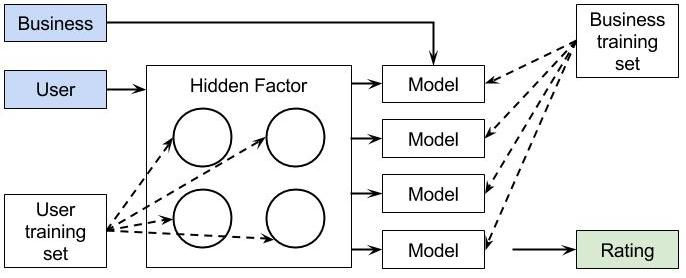
\includegraphics[width=0.9\textwidth, height=5.75cm]{architecture}
    \caption{The architecture for the overall system. Inputs are colored blue while the output is shown in green. Dotted lines represents inputs during training, and solid lines represent the flow of information at testing time. The hidden factor is used to select a model, or a mixture of models, that the business data is tested on. The output is the rating.}
    \label{fig:system}
\end{figure} 

Modeling the hidden factor in step 1 is an unsupervised learning problem, because we are constructing groups for which we have no prior labels. However, after learning the hidden factor, the step 2 is fully supervised because we are presented with a full list of ratings for each business. Considering the full system, we see that we can perform an end-to-end test given a user, a business, and an expected rating. This allows us to indirectly supervise the hidden factor to determine the appropriate hyperparameters for step 1. The overall complexity of our system grows, and we perform a train-validate-test strategy recursively for step 2 within the context of the overall system.

In the next sections, we discuss constructing the feature vectors that create the user and business data shown in Figure \ref{fig:system}. We describe multiple approaches to implement both factors, and describe our train-validate-testing strategy. Finally, we compare the different methodologies in terms of accuracy and computational time.

\section{Features}

A key to success in any machine learning problem is the selection of relevant features to accurately represent the data of interest. While algorithms are important, the success that can be achieved is often bounded by the ability of the features to accurately represent the problem. In our project, we need to develop two sets of features. The first set of features corresponds to user attributes that will be used to predict the hidden class associated with each user. The second set corresponds to business attributes that will be used to predict how a user in a given class will rate a restaurant.

\subsection{User Data}
The Yelp dataset is comprised of three relevant files: a user review file, a user attribute file, and a business attribute file. A straightforward approach would be to classify a user based purely off the data presented in the user attribute file. This file contains information about the user along with a user ID. However, the information provided is only basic with attributes such as the total number of reviews a user has written, the average of the user's ratings, and less relevant attributes such the user's full name.

Therefore, we use a different approach to form user features. We still take a couple features from the user attribute file, namely the user's average rating and the total number of reviews, but most features are formed by cross referencing the user's ID with the user reviews file. With our approach, we find the reviews associated with the user's ID and store the rating and business ID associated with each review. Then from the business ID we can cross reference the business file to determine what type fo restaurant with which it is associated.  Yelp lists categories associated with each business. For instance, every restaurant will have the string 'restaurant' in its categories but might also have the string 'Mexican restaurant.'

This allows us to form features that describe how a user prefers different types of restaurants. In particular, there is a feature associated with the user's average rating for restaurants in each category along with another feature for the number of reviews a user has given for each category. To compensate for users that preferentially give good or bad reviews, the user's average rating is subtracted from the category-averaged rating. Therefore these features provide information on the user's preferences in restaurants, such as liking Italian food but disliking Mexican food.

One major challenge with this approach is missing data. For the vast majority of users, there will be categories in which the user has given no reviews. For most machine learning algorithms, the data needs to be complete. To remedy this, the maximum likelihood estimate is chosen to fill missing data. For the case of no reviews in a given category, we take the user's average review as the maximum likelihood estimate. Since we subtract by the user's average review in category ratings, this corresponds to inserting zeros for these missing features. 

The user feature vector contains 33 features, 28 of which are associated with the average rating and number of reviews for 14 categories of restaurants. The remaining 5 features are statistical features associated with the user, such as variance of review ratings and average review rating.

\subsection{Business Data}

\section{Methodology}
\subsection{Hidden Factor}
\subsubsection{K-Means Clustering}
\subsubsection{K-Neighbors}
\subsubsection{Mixture of Gaussians}
\subsection{Second Factor}
\subsubsection{MLE}
\subsubsection{Lasso}
\subsubsection{Bayesian Ridge}
\subsubsection{Random Forests}

\section{Experiments}
\subsection{Setup}
\subsection{Results}

% \subsection{Regression}
% \subsubsection{Maximum Liklihood Estimate}
% \subsubsection{Bayesian Ridge}
% \subsubsection{Lasso}
% \subsubsection{Random Forest}

\section{References}

\end{document}
